% =========================================================
% 6.4 DISEÑO DE BASE DE DATOS
% El \section{} de esta sección está en el chapter.tex del capítulo;
% sus referencias van en seccion6_4.bib (misma carpeta).
% =========================================================

\subsection{Modelo entidad-relación}

La Figura~\ref{fig:er_db_usuarios} muestra
el modelo de la base de datos \texttt{db\_usuarios\_app}.

\clearpage
\newgeometry{margin=1cm}
\begin{landscape}
\begin{figure}[H]
    \centering
    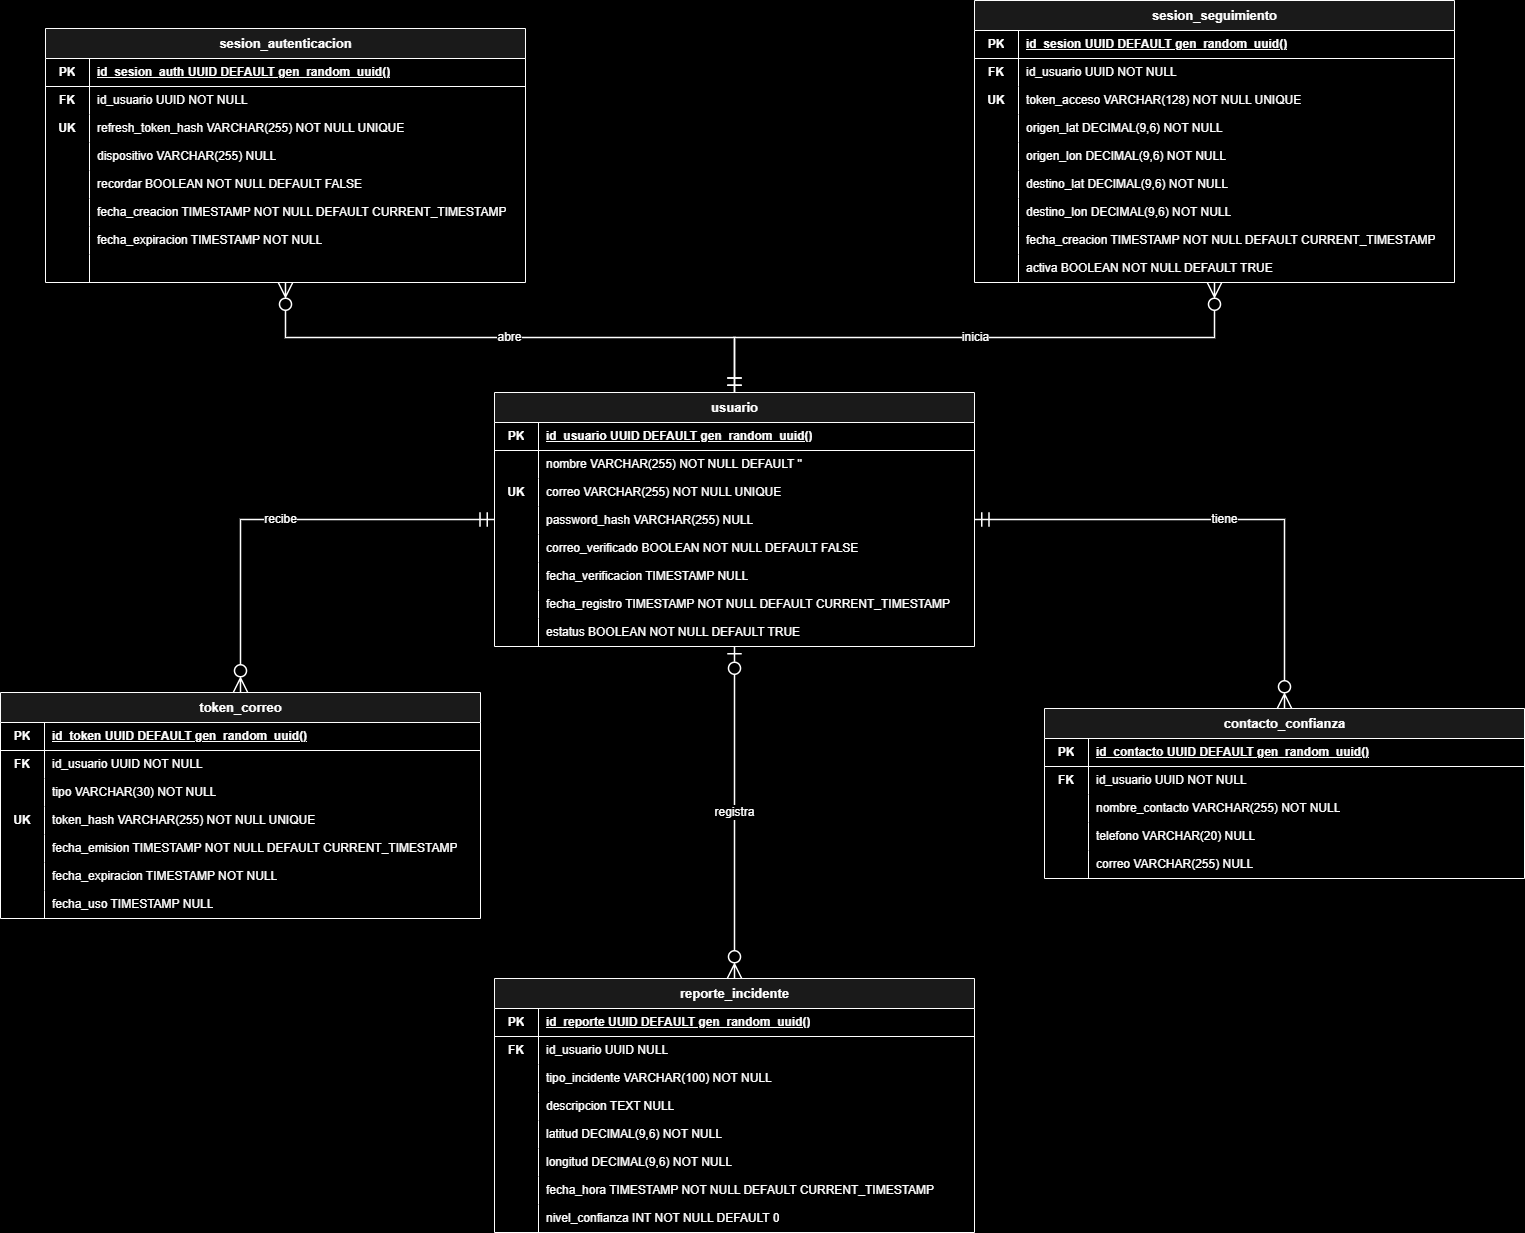
\includegraphics[width=\linewidth,
                     height=\dimexpr\textheight-2.5cm\relax,
                     keepaspectratio]{figures/capitulo6_diseno_sistema/6.4_Diseno_de_base_de_datos/BD_E-R_prototipo.png}
    \caption{Modelo entidad-relación de la base de datos \texttt{db\_usuarios\_app}.}
    \label{fig:er_db_usuarios}
\end{figure}
\end{landscape}
\restoregeometry




\subsection{Estructura y persistencia de la red de grafos}
